\documentclass[main.tex]{subfiles}
\begin{document}

\subsection{Architecture}
The system consists of several parts:

\begin{figure}[htbp!]
    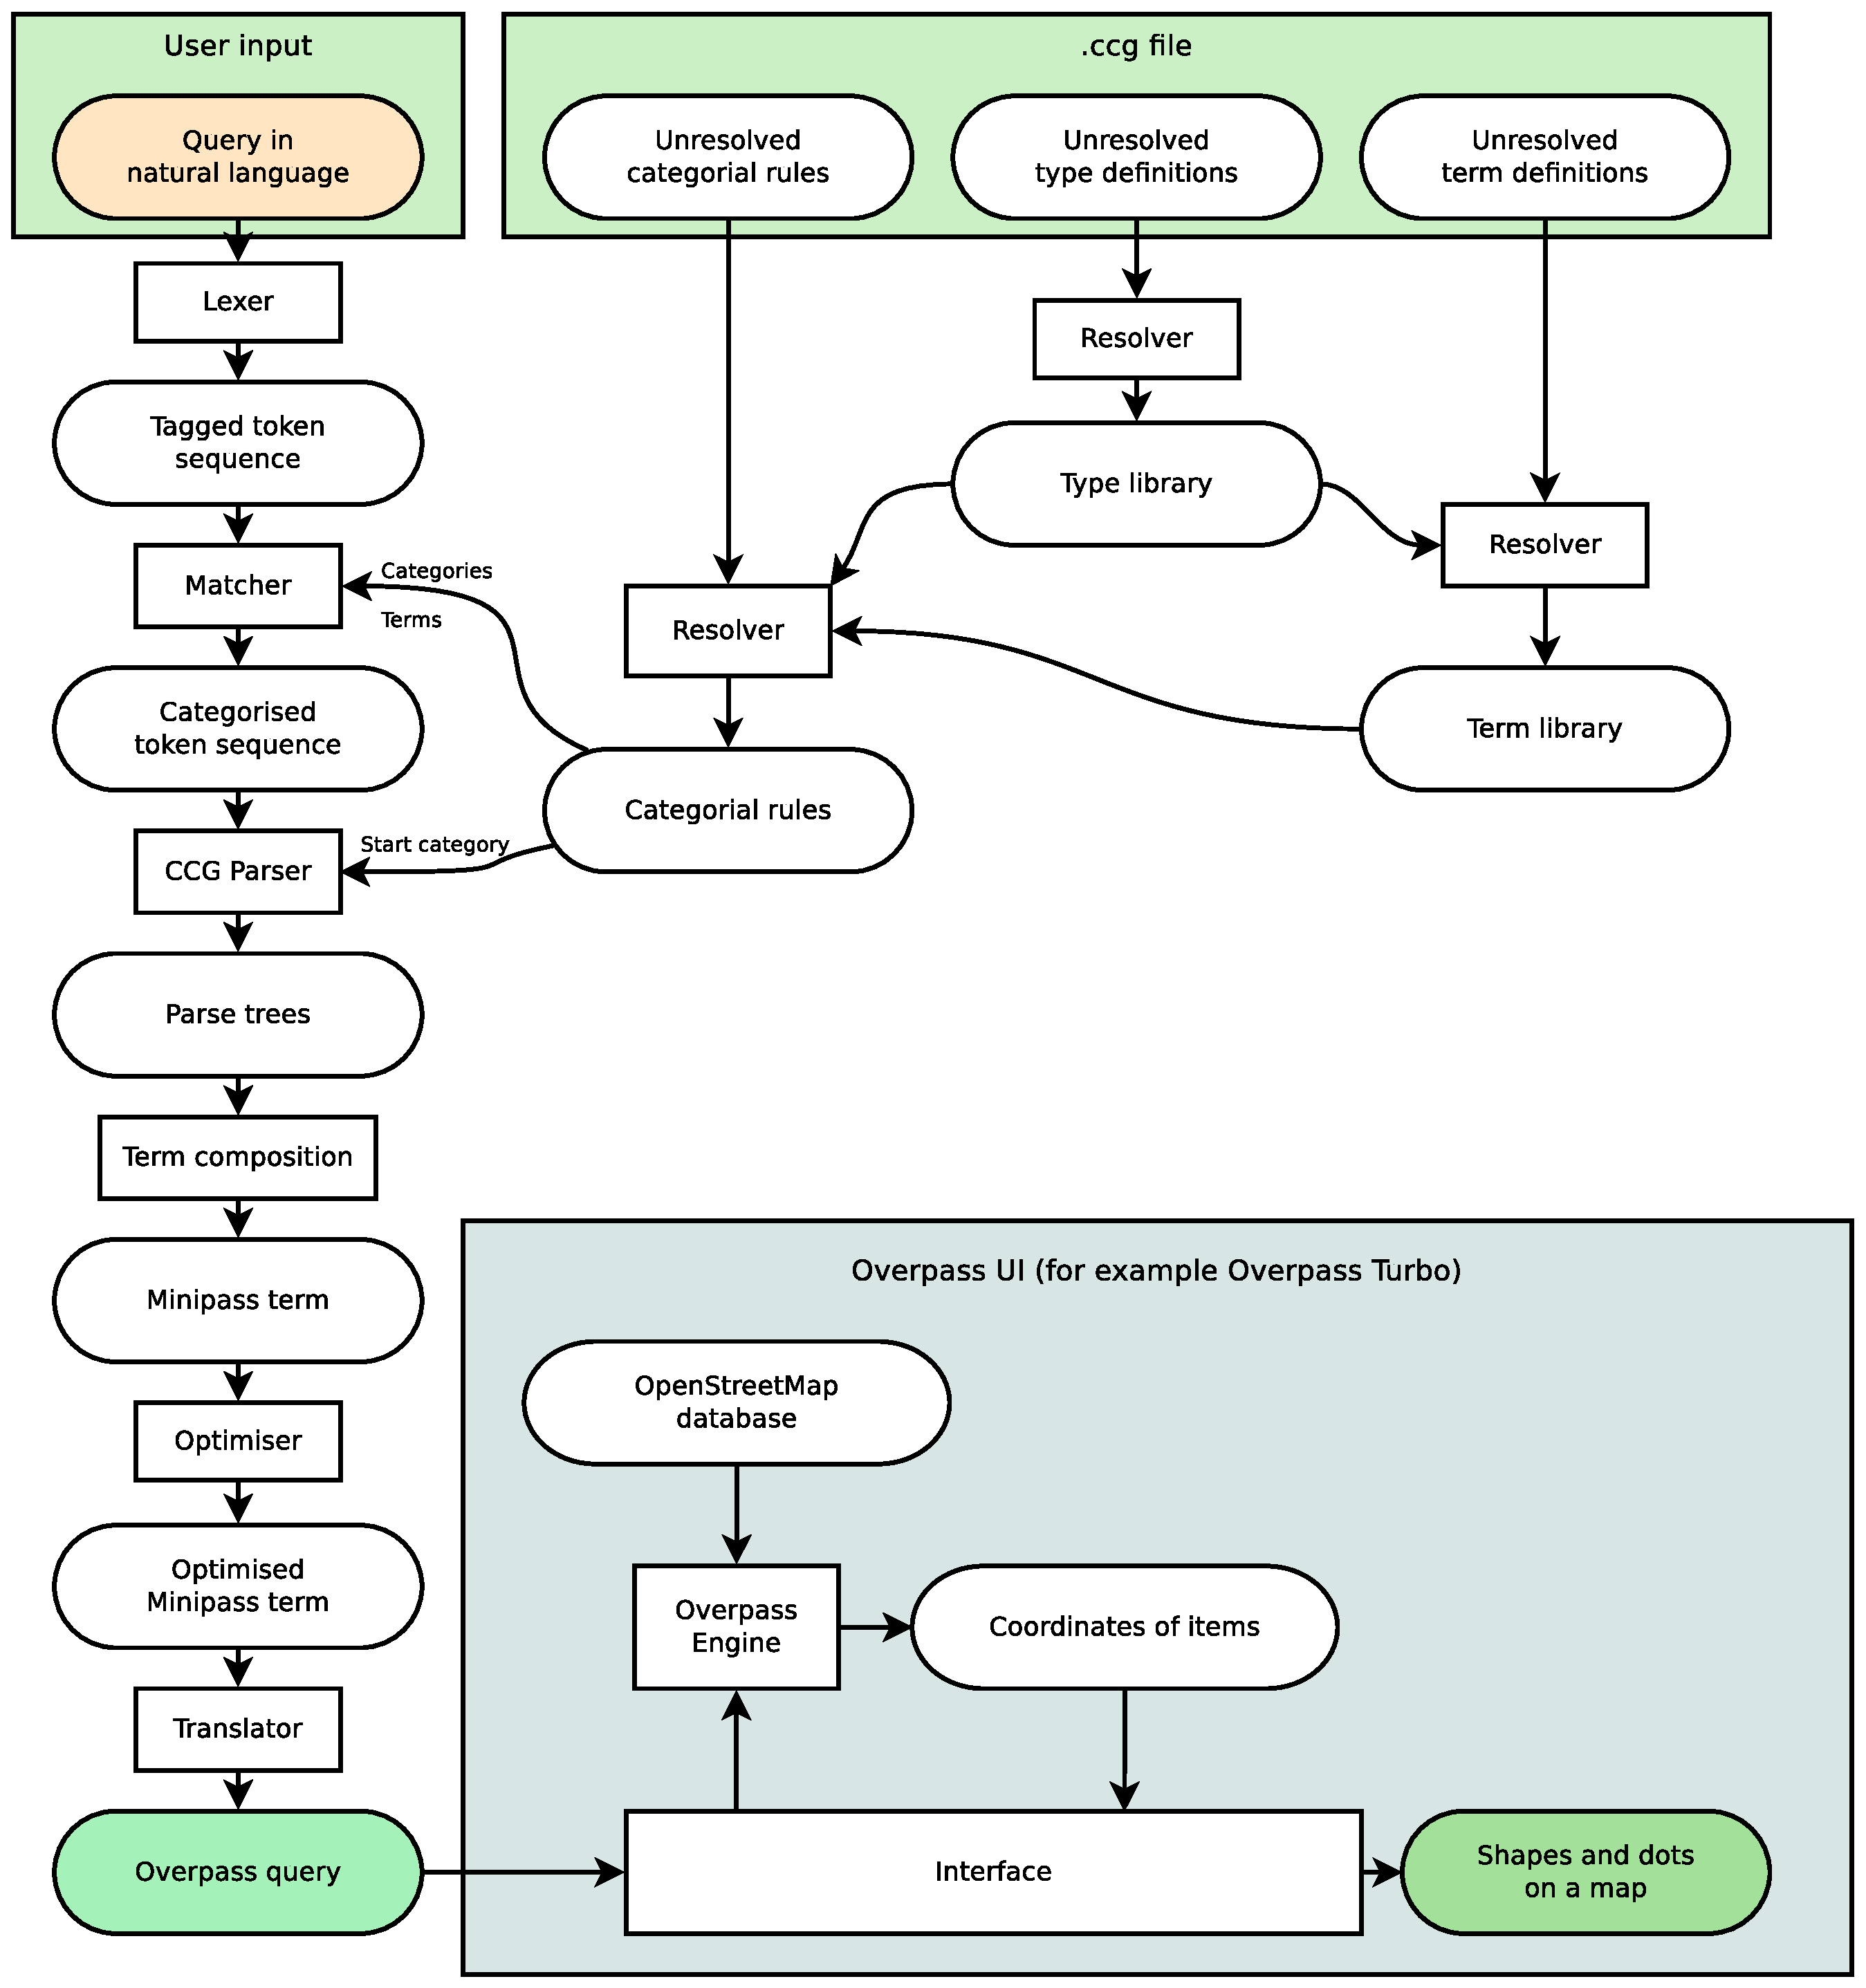
\includegraphics[width=\textwidth]{arch.eps}
    \caption{Architecture overview}
    \label{arch}
\end{figure}

\begin{itemize}
    \item Generic CCG definition language: a language for defining CCGs and
          their respective type systems and term libraries. Can be used
          standalone (for specifying CCGs which output raw parse trees)
          or by embedding a lambda calculus-based language (for specifying
          CCGs which output lambda terms)

    \item CCG Rule Matcher: a module which tags tokens from the input stream
          with Categories based on the CCG rules (defined in the CCG definition
          language)

    \item CCG Parser: a simple proof-of-concept parser based on the CYK
          algorithm

    \item English Lexer: a tokeniser, POS-tagger and lemmatiser for English
          (largely consists of external components)

    \item The Minipass language: a small, lambda calculus-based language
          which translates to Overpass, designed to be easily generated and
          to represent Overpass operators as operations on a graph.

    \item Minipass to Overpass translator: a translator from Minipass terms
          to Overpass queries which does some basic optimisations
\end{itemize}

An architecture overview can be seen at Figure \ref{arch}.

\end{document}
